
\subsection{Embedding approach metric}
In this section, the goal is to measure at each time the accuracy of detected
similarities compared to the validated ones (in the labelled similarities
dataset), with changing the embedding model and the embedding approach.

\begin{multicols}{2}
    \textbf{The embedding models:}
    \begin{itemize}
        \item \href{https://tfhub.dev/google/universal-sentence-encoder/4}
              {Universal Sentence Encoder Multilingual} (\acrshort{usem})
        \item
              \href{https://huggingface.co/sentence-transformers/paraphrase-multilingual-MiniLM-L12-v2}
              {Paraphrase Multilingual}
        \item
              \href{https://tfhub.dev/google/nnlm-en-dim50-with-normalization/2}
              {Neural-Net Language Models} (\acrshort{nnlm})
        \item Sentence transformer:
              \href{https://huggingface.co/sentence-transformers/distiluse-base-multilingual-cased-v2}
              {distiluse-base-multilingual}
    \end{itemize}
    \columnbreak
    \textbf{The embedding approaches:}
    \begin{itemize}
        \item \textbf{Approach 1}: (or Concatenate and embed) Concatenate the texts and do the embeddings
        \item \textbf{Approach 2}: (or Concatenate embeddings) Perform the embedding per cell and concatenate the results.
        \item \textbf{Approach 3}: (or PCA on embeddings) Perform the embedding per cell, reduce their dimension with
              \acrshort{pca} and concatenate.
        \item \textbf{Approach 4}: (or Mean on embeddings) Perform the embedding per cell, and get the mean for each
              component in the result embedding vectors.
    \end{itemize}
\end{multicols}

To compute this accuracy, we represent the estimated similarities between couples
of datasets in a form of a matrix where each axis represents a dataset column. The
next step is to compute for each dataset couple the accuracy of the estimated
similarities between the columns that have been labelled similar.

To define this metric mathematically, let $E$ be the estimation matrix, and  $L$
be the labelled similarity matrix, and $1_L$ the number of occurrences of 1 in $L$

\begin{equation}
    metric = \frac{1}{1_L} \sum_i \sum_j L_{i,j} * E_{i,j}
\end{equation}

The figure \ref{fig:tests_embedding_metric} shows an example of two datasets
with 4 and 5 columns respectively.

\begin{figure}[h]
    \centering
    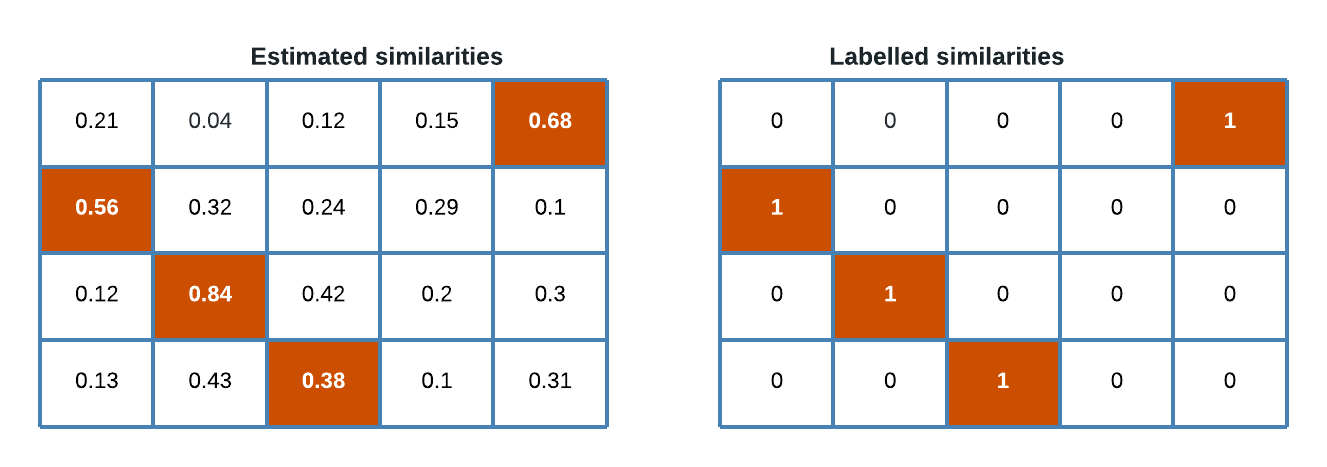
\includegraphics[width=\textwidth]{tests/embedding_metric.png}
    \caption{Embedding metric computing example}
    \label{fig:tests_embedding_metric}
\end{figure}

The metric in this case is calculated by picking up the similarities
corresponding to labelled similarities and computing their means:
\begin{equation}
    metric = \frac{1}{4} (0.68 + 0.56 + 0.84 + 0.38) = 0.615
\end{equation}

The table \ref{table:embedding_metric_result} presents the results of this test
with every combination of embedding model with an embedding approach.

\hspace{1cm}

\begin{table}[h]
    \begin{center}
        \begin{tabular}{|c | c | c | c| c|}
            \hline
                                            & \textbf{\acrshort{usem}}         &
            \textbf{\acrshort{nnlm}}        & \textbf{Paraphrase Multilingual} &
            \textbf{Distiluse}
            \\
            \hline

            \textbf{Concatenate and embed}  & 0.301                            & 0.580
                                            & 0.409                            & 0.365
            \\
            \hline

            \textbf{Concatenate embeddings} & 0.044                            & 0.06  &
            0.085                           & 0.107                                      \\
            \hline

            \textbf{PCA on embeddings}      & 0.275                            & 0.319
                                            & 0.403                            & 0.350
            \\
            \hline

            \textbf{Mean on embeddings}     & 0.494                            & 0.583
                                            & 0.572                            & 0.554
            \\
            \hline
        \end{tabular}
    \end{center}
    \caption{Results for the embedding choice metric}
    \label{table:embedding_metric_result}
\end{table}
Some remarks can be done over these results:
\begin{itemize}
    \item The best accuracies were around $0.56, 0.58$.
    \item The fourth approach gave the best results for each embedding model.
    \item The notion of angular distance loses its sense when the dimensions are
          too big case of approach 2 (Concatenate embeddings). As each cell with
          this approach will be in a dimension of 512 or 368 (depending on the
          embedding model used), the vector of concatenated word representations
          will become too large, which will make the angular metric lose some
          relevance, and also the concatenation of the embeddings won't give a
          good comprehension of the column content.
    \item The accuracies depend on the embedding model understanding of
          different forms of texts, as there may be some forms that are not
          understandable, for example: links, email addresses, acronyms, ect..

\end{itemize}

The configuration selected after this experiment is:
\begin{itemize}
    \item \textbf{Embedding model:} Paraphrase Multilingual
    \item \textbf{Embedding approach:} Approach 4; perform the embedding per
          cell, and get the mean for each component in the result embedding vectors.
\end{itemize}
% TODO:
% - mention in \textbf{Embedding approach metrics} the embedding section once it
%   is done.
